%\documentclass[main]{subfiles}

%\begin{document}


\section{Score-based variational inference with orthogonal function expansions}
\label{sec:scorebasedVI}

In this section we use orthogonal function expansions to develop new variational families for
approximate probabilistic inference. In \Cref{sec:orth}, we review the basic properties of these
expansions.
In \Cref{sec:eigenVI}, we introduce a score-based divergence for VI with these families;
notably, for this divergence, the optimization for VI reduces to an eigenvalue
problem. Finally in \Cref{sec:precon},
we consider how to use these variational approximations for unstandardized distributions;
in these settings we must carefully manage the trade-off between expressiveness and
computational~cost.

%%%%%%%%%%%%

\subsection{Orthogonal function expansions}
\label{sec:orth}

Let $\mathcal{Z}\subseteq\mathbb{R}^D$ denote the support of the
target distribution $p$.
Suppose that there exists a
complete set of orthonormal basis functions
$\{\phi_k(z)\}_{k=1}^\infty$ on this set. By \emph{complete}, we mean
that any sufficiently well-behaved function
\mbox{$f:\mathcal{Z}\rightarrow\mathbb{R}$} can be approximated, to
arbitrary accuracy, by a particular weighted sum of these basis
functions, and by \emph{orthonormal}, we mean that the basis functions
satisfy
\begin{align}
\label{eq-orthonormal}
  \int\!\phi_k(z)\phi_{k'}(z)\, dz =
  \left\{
  \begin{array}{rr} 1 & \mbox{if $k=k'$}, \\
    0 & \mbox{otherwise,}\end{array}\right.
\end{align}
where the integral is over $\mathcal{Z}$.
Define the
$K^\text{th}$-order variational family $\mathcal{Q}_K$ to be the set containing
all distributions of the form
\begin{align}
  q(z) =  \left(\sum_{k=1}^{K} \alpha_k \phi_k(z)\right)^2\quad\mbox{where}\quad\sum_{k=1}^{K} \alpha_k^2=1,
\label{eq:OF-1}
\end{align}
and where $\alpha_k\in\R$ for $k=1,\ldots, K$ are the parameters of the family $\mathcal{Q}_K.$
In words,  $\mathcal{Q}_K$ contains all distributions that can be obtained by
taking weighted sums of the first $K$ basis functions and then \textit{squaring} the result.

\Cref{eq:OF-1} involves a squaring operation, a sum-of-squares
constraint, and a weighted sum. The squaring operation ensures that
the density functions in $\mathcal{Q}_K$ are nonnegative (i.e., with
$q(z)\!\geq\!0$ for all $z\in\mathcal{Z}$), while the sum-of-squares constraint
ensures that they are normalized:
\begin{align}
  \int\! q(z)\, dz\, =\, \int\! \left(\sum_{k=1}^{K} \alpha_k \phi_k(z)\right)^2\!\! dz\, =\,
  \int\! \sum_{k,k'=1}^{K} \alpha_k \alpha_{k'} \phi_k(z)\phi_{k'}(z)\, dz\, =\, \sum_{k=1}^{K} \alpha_k^2 = 1.
\end{align}

The weighted sum in \Cref{eq:OF-1} bears a superficial similarity
to a mixture model, but note that neither the basis
functions~$\phi_k(z)$ nor the weights~$\alpha_k$ in \Cref{eq:OF-1}
are constrained to be nonnegative. Distributions of this form arise
naturally in physics from the quantum-mechanical \emph{wave functions}
that satisfy Schr\"odinger's equation \citep{griffiths2018introduction}.
In that setting, though, it is
typical to consider complex-valued weights and basis functions,
whereas here we only consider real-valued ones.


The simplest examples of orthogonal function expansions arise in one
dimension. For example, functions on the interval $[-1,1]$ can be
represented as weighted sums of Legendre polynomials, while functions
on the unit circle can be represented by Fourier series of sines and
cosines; see \Cref{tab:onedim}. Distributions on unbounded
intervals can also be represented in this way. On the real line, for
example, we may consider approximations of the form in
\Cref{eq:OF-1} where
\begin{equation}
\phi_{k+1}(z) = \left(\sqrt{2\pi}k!\right)^{-\frac{1}{2}}\left(e^{-\frac{1}{2}z^2}\right)^{\frac{1}{2}}\,\text{H}_{k}(z),
\label{eq:phi-hermite}
\end{equation}
and $\text{H}_k(z)$ are the \emph{probabilist's} Hermite polynomials given by
\begin{equation}
\text{H}_k(z) = (-1)^k e^{\frac{z^2}{2}} \frac{d^k}{dz^k}\left[e^{-\frac{z^2}{2}}\right].
\label{eq:hermite}
\end{equation}
Note how the lowest-order basis function $\phi_1(z)$ in this family gives rise
(upon squaring) to a Gaussian distribution with zero mean and unit variance.

\Cref{fig:onedim} shows how various multimodal distributions with
one-dimensional support can be approximated by computing weighted sums
of basis functions and squaring their result. We emphasize that
\textit{the more basis functions in the sum, the better the
  approximation}.

%%%%%%%%%%%%

\begin{table*}[t]
\small
%\begin{center}
    \centering
    \caption{Examples of orthogonal function expansions in one dimension. The basis functions in the
        table are not normalized, but they can be rescaled so that their squares integrate to one.
    \vspace{5pt}
    }

    \label{tab:onedim}
    \begin{tabular}{lll}
    \toprule
    \textbf{support} & \textbf{orthogonal family} & \textbf{basis functions} $\phi_k(\cdot)$  \\ [0.3ex]
    \midrule
    $z\in[-1,1]$ & Legendre polynomials & $\{1,\, z,\, 3z^2\!-\!1,\, 5z^3\!-\!3z, \ldots\}$ \\ [0.3ex]
    $z=e^{i\theta}\!\in S^1$\hspace{2ex} & Fourier basis & $\{1,\cos\theta,\sin\theta,\cos 2\theta,\sin 2\theta,\ldots\}$ \\[0.3ex]
    $z\in[0,\infty)$ & weighted Laguerre polynomials &    $e^{-\frac{z}{2}}\{1,1\!-\!z,z^2\!-\!4z\!+\!2,\ldots\}$\\ [-0.3ex]
    $z\in\mathbb{R}$ & weighted Hermite polynomials & $e^{-\frac{z^2}{4}}\{1,z,(z^2\!-\!1),(z^3\!-\!3z),\ldots\}$\\ [0.5ex]
    \bottomrule
    \end{tabular}
    %\end{center}
    \vspace{-10pt}
\end{table*}

\begin{figure}[t]
\centering
\begin{subfigure}[b]{0.325\linewidth}
    \centering
    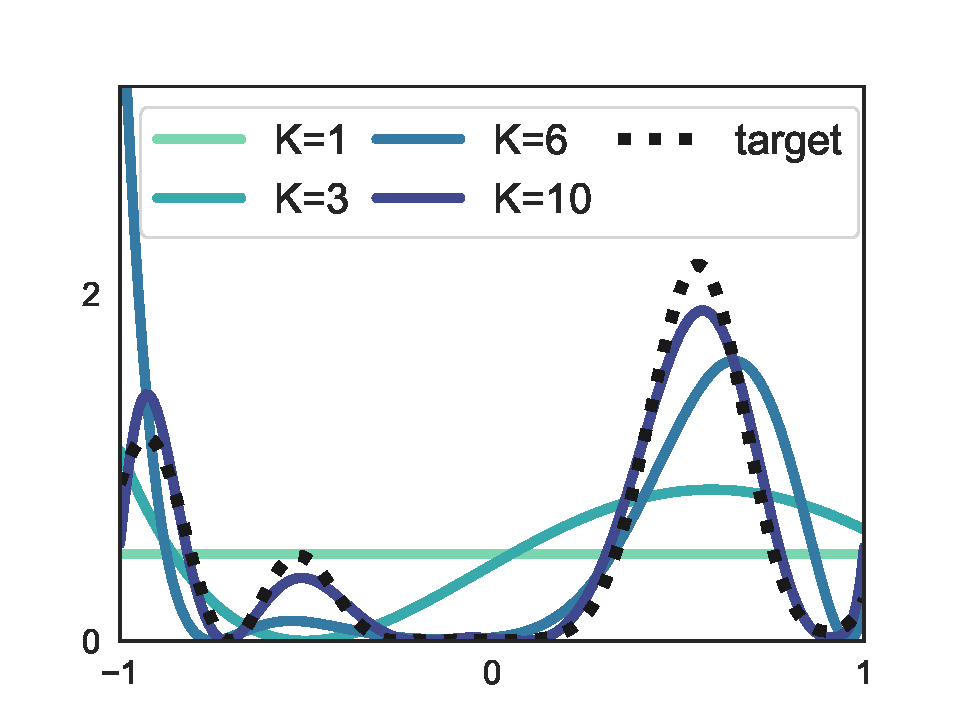
\includegraphics[scale=0.31]{figs/1d_legendre2.pdf}
    \caption{Legendre polynomial expansion}
\end{subfigure}
\begin{subfigure}[b]{0.325\linewidth}
    \centering
    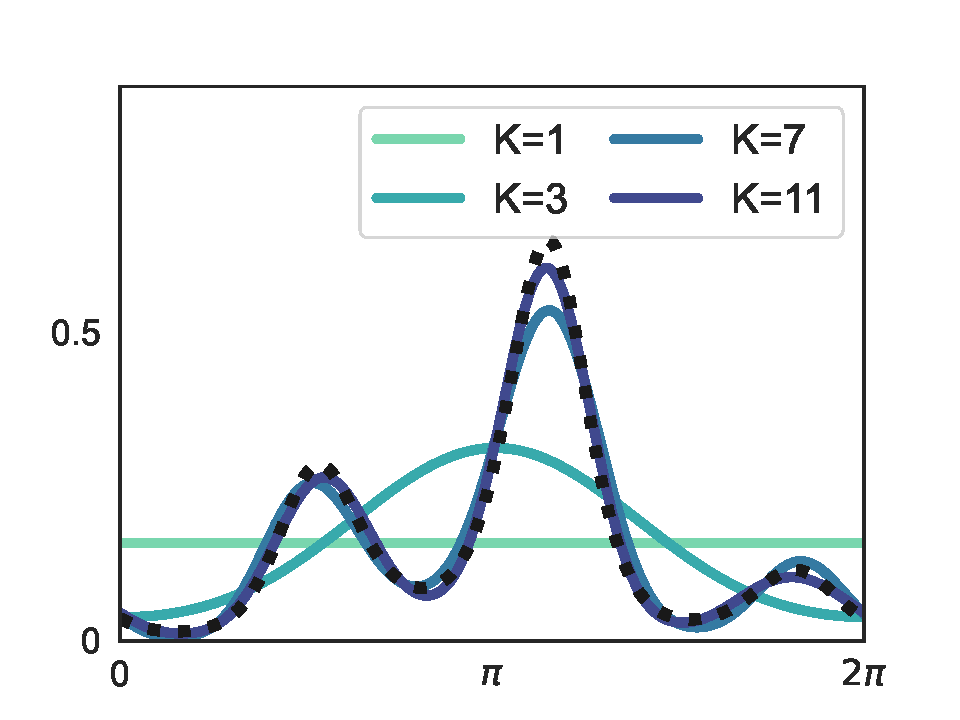
\includegraphics[scale=0.31]{figs/1d_fourier2.pdf}
    \caption{Fourier series expansion}
\end{subfigure}
\begin{subfigure}[b]{0.325\linewidth}
    \centering
    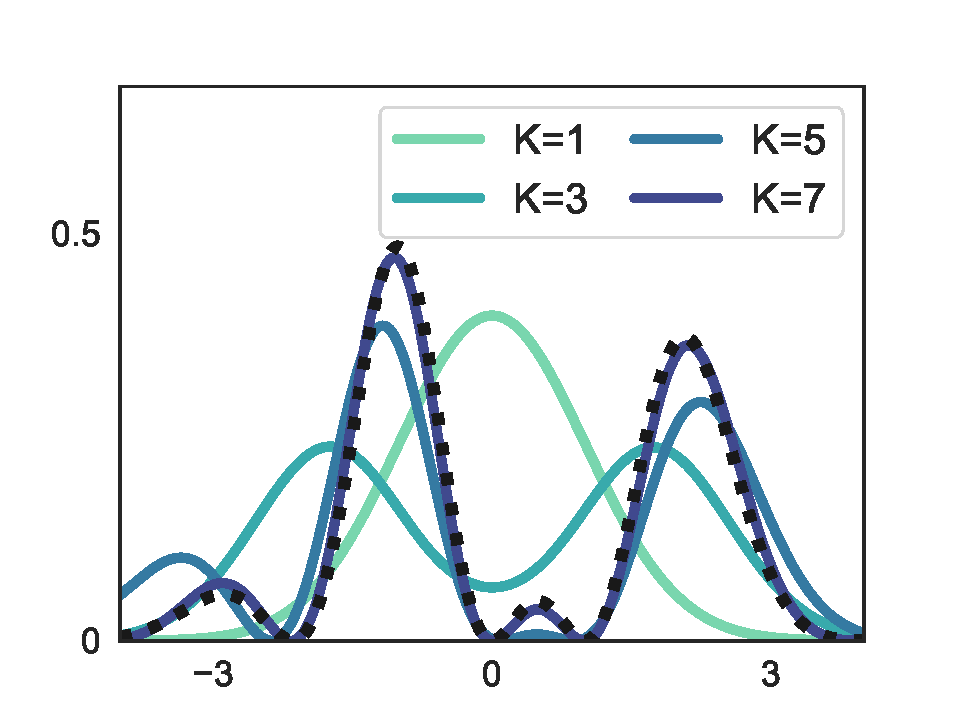
\includegraphics[scale=0.31]{figs/1d_hermite2.pdf}
    \caption{Hermite polynomial expansion}
    \label{fig:onedim:c}
\end{subfigure}
\caption{Target probability distributions (black dashed curves) on the interval $[-1,1]$ (left), the unit circle (middle), and the
    real line (right), and their approximations by orthogonal function expansions
    from different families and of different orders; see \Cref{eq:OF-1} and \Cref{tab:onedim}.}
\vspace{-15pt}
\label{fig:onedim}
\end{figure}

%%%%%%%%%%%%%

Orthogonal function expansions in one dimension are also important because their Cartesian products can be used to generate orthogonal function expansions in higher dimensions. For example, we can approximate distributions over (say) $\mathbb{R}^3$ by
\begin{equation}
q(z_1,z_2,z_3) =  \left(\sum_{i=1}^{K_1}\sum_{j=1}^{K_2}\sum_{k=1}^{K_3} \beta_{ijk}\, \phi_i(z_1)\phi_j(z_2)\phi_k(z_3)\right)^2\quad\mbox{where}\quad \sum_{ijk}\beta^2_{ijk} = 1,
\label{eq:3d}
\end{equation}
where $\beta_{ijk}\in \R$ now parametrize the family.
Note that there are a total $K_1 K_2 K_3$ parameters in the above expansion, so that this method of
Cartesian products does not scale well to high dimensions if multiple basis functions are used per
dimension.
Note that the same strategy can also be used for random variables of
mixed type: for example, from \Cref{tab:onedim}, we can create a variational family of distributions over $\mathbb{R}\!\times\![-1,1]\!\times\![0,\infty)$ from the Cartesian product of orthogonal function expansions involving Hermite, Legendre, and Laguerre polynomials.

As shown in \Cref{fig:onedim}, the approximating distributions
from $K^\text{th}$-order expansions can model the presence of multiple
modes as well as many types of asymmetry, and this expressiveness also
extends to higher dimensions. Nevertheless, it remains tractable to
sample from these distributions and even to calculate (analytically)
their low-order moments, as we show in \Cref{app:sampling,app:moments}.

For concreteness, consider the distribution over $\mathbb{R}^3$ in
\Cref{eq:3d}. The marginal distribution $q(z_1)$ is
\begin{align}
q(z_1) = \int\! q(z_1,z_2,z_3)\,dz_2\, dz_3 = \sum_{ii'} \left[\sum_{jk} \beta_{ijk}\beta_{i'jk}\right] \phi_i(z_1)\phi_{i'}(z_1),
\label{eq:marginal}
\end{align}
and from this expression, moments such as $\mathbb{E}[z_1]$
%(\Cref{eq:Amu})
and
$\text{Var}[z_1]$
%(\Cref{eq:Anu})
can be calculated by evaluating integrals involving
the elementary functions in \Cref{tab:onedim}.
(In practice,
these integrals are further simplified by recursion relations that
relate basis functions of different orders;
we demonstrate how to compute the first two moments for
the normalized Hermite family in
\Cref{eq:mom1ij,eq:mom2ij}.)

To generate samples $\{z^{(t)}\}$, each dimension is sampled as follows:
we draw
$z_1^{(t)} \sim q(z_1)$ by computing the cumulative distribution function (CDF)
of this marginal distribution and then numerically inverting this CDF.
Finally, extending these ideas, we can calculate higher-order moments
and obtain joint samples via the nested draws
\begin{align}
\label{eq:sample}
    z_1^{(t)} \sim q(z_1),\quad z_2^{(t)} \sim q(z_2 \given z_1),\quad
    z_3^{(t)} \sim q(z_3  \given z_1,z_2).
\end{align}
The overall complexity of these procedures scales no worse than
quadratically in the number of basis functions in the expansion. These
extensions are discussed further in \Cref{app:sampling,app:moments}.

%%%%%%%%%%%

\subsection{EigenVI}
\label{sec:eigenVI}

In variational inference, we posit a parameterized family of
approximating distributions and then compute the particular approximation
in this family that is closest to a target distribution of interest.
\Cref{eq:OF-1}
constructs a variational family $\Q_K$ from the orthogonal functions $\{\phi_k(z)\}_{k=1}^K$ whose variational parameters are the weights
$\{\alpha_k\}_{k=1}^{K}$. We now derive \textit{EigenVI}, a method to find
$q \in \Q_K$ that is close to the target distribution $p(z)$.

We first define the measure of closeness that we will minimize.
EigenVI measures the quality of an approximate density by the
\textit{Fisher divergence} \citep{hyvarinen2005estimation},
\begin{align}
\label{eq-divergence}
    \D(q,p) = \int \norm{\nabla \log q(z) - \nabla\log p(z)}^2 q(z) dz,
\end{align}
where $\nabla \log q(z)$ and $\nabla \log p(z)$ are the score functions of the
variational approximation and target, respectively. Suppose that $q$ and $p$ have the same support; then the Fisher divergence vanishes if and only if the scores of $q$ and $p$ are
everywhere equal.

Though $p$ is, by assumption, intractable to compute, in many applications it is
possible to efficiently compute the score $\nabla \log p$ at any point
$z\in\mathcal{Z}$. For example, in Bayesian models the score of the target
posterior is equal to the gradient of the log joint. This observation is the main
motivation for score-based methods in probabilistic
modeling~\citep{liu2016stein,yu2023semiimplicit,modi2023,cai2024}.

Here we seek the $q\!\in\!\Q_K$ that minimizes $\D(q,p)$. But now a
challenge arises: it is generally difficult to evaluate the integral
for $\D(q,p)$ in \Cref{eq-divergence}, let alone to minimize it as a
function of~$q$.
While it is possible to sample from the distribution $q$,
it is not straightforward to simultaneously sample from $q$ and optimize over the variational parameters $\{\alpha_k\}_{k=1}^K$ in terms of which it is defined.
Instead, we construct an unbiased estimator of
$\D(q,p)$ by importance sampling, which also decouples the sampling distribution from the optimization.
Let $\{z^1,z^2,\ldots z^B\}$ denote a
batch of $B$ samples drawn from some proposal distribution $\pi$ on
$\mathcal{Z}$. From these samples we can form the unbiased estimator
\begin{align}
  \label{eq-empirical-divergence}
  \widehat\D_{\pi}(q, p) =
  \sum_{b=1}^B \frac{q(z^b)}{\pi(z^b)} \, \big\|\nabla \log q(z^b) - \nabla\log p(z^b)\big\|^2.
\end{align}
This estimator should be accurate for appropriately broad proposal
distributions and for sufficiently large batch sizes. We can therefore
attempt to minimize \Cref{eq-empirical-divergence} in place of
\Cref{eq-divergence}.

Now we show that the minimization of \Cref{eq-empirical-divergence} over
$q\in\Q_K$ simplifies to a minimum eigenvalue problem for the weights
$\{\alpha_k\}_{k=1}^{K}$.
To obtain the eigenvalue problem, we substitute the
orthogonal function expansion in \Cref{eq:OF-1}
into \Cref{eq-empirical-divergence} for the unbiased estimator of
$\D(q,p)$. As an intermediate step, we differentiate
\Cref{eq:OF-1} to obtain the scores
\begin{equation}
\label{eq:scores}
\nabla\log q(z^b) = \frac{2\sum_k \alpha_k \nabla \phi_k(z^b)}{\sum_k \alpha_k \phi_k(z^b)}.
\end{equation}
Further substitution of the scores provides the key result behind our
approach: the unbiased estimator in
\Cref{eq-empirical-divergence} is a simple quadratic form in the
weights $\alpha := [\alpha_1,\ldots,\alpha_K]^\top$ of the orthogonal function expansion,
\begin{equation}
\widehat\D_{\pi}(q,p) =
\alpha^\top\! M\alpha,
\label{eq:quadform}
\end{equation}
where the coefficients of the quadratic form are given by
\begin{equation} \label{eq:M}
  M_{jk} = \sum_{b=1}^B\frac{1}{\pi(z^b)}
    \left[2\nabla \phi_j(z^b) - \phi_j(z^b)\nabla\log p(z^b)\right]\cdot\left[2\nabla \phi_k(z^b) -
    \phi_k(z^b)\nabla\log p(z^b)\right].
\end{equation}
Note that the elements of the $K\!\times\! K$ symmetric matrix $M$ capture all of the dependence on
the batch of samples $\{z^b\}_{b=1}^B$, the scores of $p$ and $q$ at these samples,
and
the choice of the family of orthogonal functions.
Next we minimize the quadratic
form in \Cref{eq:quadform} subject to the sum-of-squares
constraint $\sum_k \alpha_k^2 = 1$ in \Cref{eq:OF-1}.
In this way we obtain the eigenvalue problem~\citep{courant1924methoden}
\begin{align}
  \label{eq:eigenVI-solution}
\min_{q\in\Q_K}\left[\widehat{\D}_{\pi}(q,p)\right] =
  \min_{\|\alpha\|=1}
  \left[\alpha^\top M\alpha\right] =:
  \lambda_{\text{min}}(M),
\end{align}
where $\lambda_{\text{min}}(M)$ is the minimal eigenvalue of $M$,  and the
optimal weights are given (up to an arbitrary sign) by its
corresponding eigenvector; see \Cref{app:eigen} for a proof.
EigenVI solves \Cref{eq:eigenVI-solution}.

We note that the eigenvalue problem in EigenVI arises from the curious alignment of three particular choices---namely, (i) the choice of variational family
(based on orthogonal function expansions), (ii) the choice of
divergence (based on score-matching), {and (iii) the choice of estimator for the divergence
(based on importance sampling)}.
The simplicity of this eigenvalue problem stands
in contrast to the many heuristics of gradient-based optimizations---involving learning
rates, terminating criteria, and perhaps other algorithmic
hyperparameters---that are typically required for ELBO-based
BBVI~\citep{dhaka2020robust,dhaka2021challenges}.
But EigenVI is also not entirely free of heuristics; to compute the estimator in
\Cref{eq-empirical-divergence} we must also specify the proposal distribution $\pi$ and the number
of samples $B$; see \Cref{sec:discussion:eigenvi} for a discussion.

The size of the eigenvalue problem in EigenVI is equal to the
number of basis functions $K$ in the orthogonal function expansion of \Cref{eq:OF-1}. The
eigenvalue problem also generalizes to orthogonal function expansions
that are formed from Cartesian products of one-dimensional families,
but in this case, if multiple basis functions are used per dimension,
then the overall basis size grows exponentially in the dimensionality.
Thus, for example, the eigenvalue problem would be of size
$K_1 K_2 K_3$ for the approximation in \Cref{eq:3d}, as can be
seen by ``flattening'' the tensor of weights $\beta$ in \Cref{eq:3d}
into the vector of weights $\alpha=\textbf{vec}(\beta)$ in \Cref{eq:OF-1}.
Finally, we note that EigenVI only needs to compute the minimal eigenvector of $M$ in \Cref{eq:eigenVI-solution}, and therefore it can benefit from specialized routines that are much less expensive than a full diagonalization.




\subsection{EigenVI in $\reals^D$:\ the Hermite family and standardization}
\label{sec:precon}

We now discuss the specific case of EigenVI for $\mathcal{Z}\!=\!\reals^D$ with the Hermite-based variational family in \Cref{eq:phi-hermite}.
For this case, we propose a transformation of the domain that serves to precondition or \textit{standardize}
the target distribution before applying EigenVI.
While this standardization is not required to use EigenVI,
it  helps to reduce the number of basis functions needed to approximate the target,
leading to a more computationally efficient procedure.
It also suggests natural default choices for the
proposal distribution $\pi$ in \Cref{eq-empirical-divergence}.

Recall that the eigenvalue problem grows linearly in size with the number of basis functions. Before applying EigenVI, our goal is therefore to transform the domain in a way that reduces the number of basis functions needed for a good approximation.
To meet this goal for distributions over $\reals^D$, we observe that the lowest-order basis function of the Hermite family in \Cref{eq:phi-hermite} yields (upon squaring) a standard multivariate Gaussian, with zero mean and unit covariance.
Intuitively, we might expect the approximation of EigenVI to require fewer basis functions if the statistics of the target distribution nearly match those of this lowest-order basis function. The goal of standardization is to achieve this match, to whatever extent possible, by a suitable transformation of the underlying domain. Having done so, EigenVI in $\reals^D$ can then be viewed as
a systematic framework to model non-Gaussian effects via a small number of higher-order terms in its orthogonal function expansion.

Concretely, we consider a linear transformation  of the domain:
\begin{align}
    \tilde{z} =
    %\T(z) =
    \Sigma^{-\frac{1}{2}}(z\!-\!\mu),
\end{align}
where $\mu$ and $\Sigma$ are  estimates of the mean and covariance
obtained
from some other algorithm
(e.g., a Laplace approximation,  Gaussian variational inference,  Monte Carlo, or domain-specific
knowledge).
We then apply the EigenVI to fit a $K$th-order variational approximation $\tilde q(\tilde z)$
to the target distribution $\tilde{p}(\tilde{z})$ that is induced by this transformation;
afterwards, we reverse the change-of-variables to obtain the final approximation to $p(z)$, i.e.,
\begin{align}
q(z) = \tilde{q}(\tilde{z})|\Sigma|^{-1/2}.
\end{align}

\Cref{fig:standardize} shows why it is more difficult to approximate distributions that are
badly centered or poorly scaled. The left panel shows the effect of translating a standard Gaussian
\textit{away} from the origin and \textit{shrinking} its variance; note how a comparable
approximation to the uncentered Gaussian now requires a 16th-order expansion.
On the other hand, after standardization, the target
can be perfectly fitted by the base distribution
in the orthogonal family of reweighted Hermite polynomials.
%
The right panel shows
the similar effect of translating the mixture distribution in \Cref{fig:onedim} (right panel);
comparing these panels, we see that twice as many basis functions ($K\!=\!14$ versus $K\!=\!7$)
are required to provide a comparable fit of the uncentered mixture.


\begin{figure}
\centering
\begin{subfigure}[b]{0.40\linewidth}
    \centering
    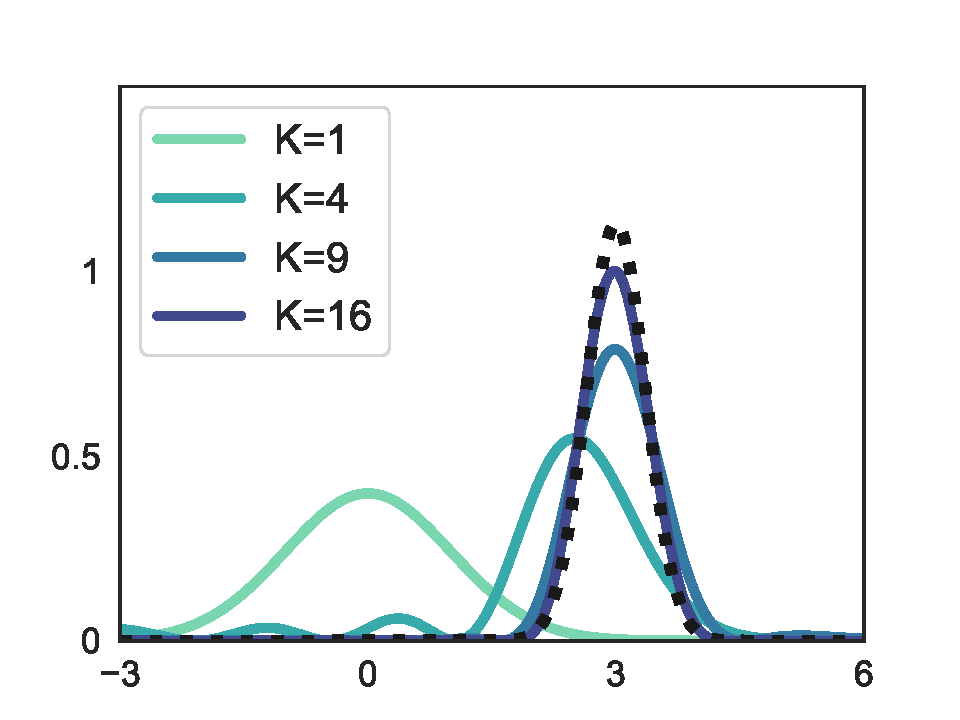
\includegraphics[scale=0.31]{figs/1d_precond_gauss2.pdf}
    \caption{Gaussian target, mean $3$ and variance $\frac{1}{8}$}
\end{subfigure}
\begin{subfigure}[b]{0.40\linewidth}
    \centering
    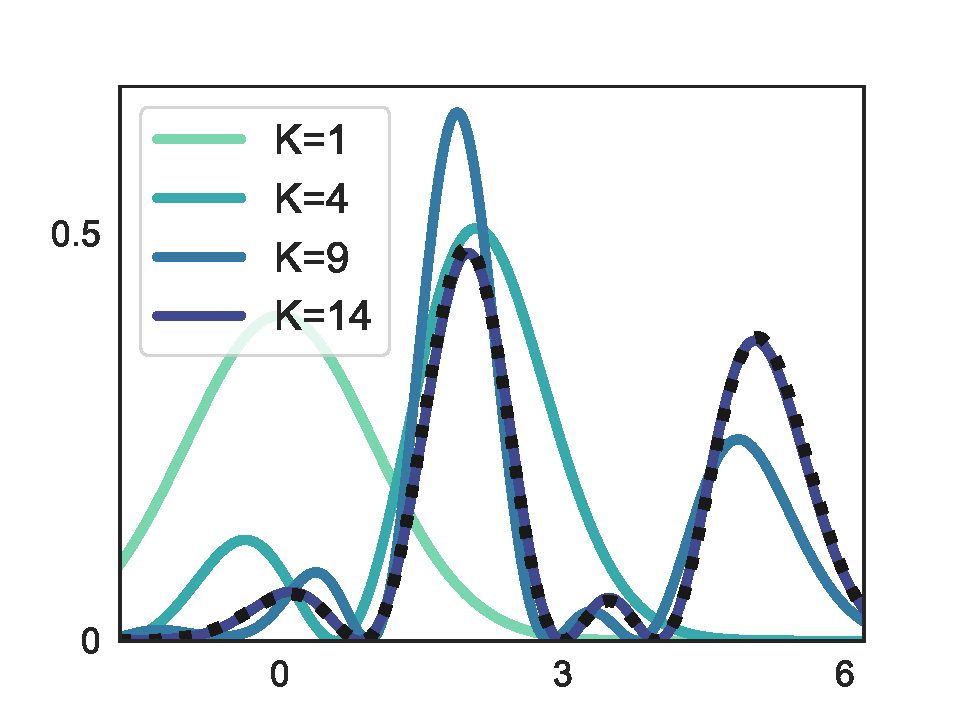
\includegraphics[scale=0.31]{figs/1d_precond_mixture2.pdf}
\caption{Mixture target (translation of \Cref{fig:onedim:c})}
\end{subfigure}
    \caption{Higher-order expansions may be required to approximate target distributions
(black)
    that are not standardized. \textit{Left:} approximation of a non-standardized Gaussian.
    \textit{Right:} approximation of the mixture distribution
    in \Cref{fig:onedim} after translating its largest modes away from the origin.
}
\label{fig:standardize}
\vspace{-13pt}
\end{figure}

Finally, we note another benefit of standardizing the target before fitting EigenVI; when the target has nearly zero mean and unit covariance, it becomes simpler to identify natural choices for the proposal distribution $\pi$.
Intuitively, in this case, we want a proposal distribution that has the same mean but heavier tails than a standard Gaussian.
In our experiments, we use two types of centered proposal distributions---uniform and isotropic Gaussian---whose variances are greater than one.


%\end{document}


%%% Local Variables:
%%% mode: latex
%%% TeX-master: "main"
%%% End:
